\documentclass{oblivoir}
\usepackage{amsmath,amssymb,kotex,kswrapfig,mdframed,tabto,enumitem,graphicx}

\usepackage{tabu,multirow}

%%% Counters
\newcounter{num}

%%% Commands
\newcommand\defi[1]
{\bigskip\par\noindent\stepcounter{num} \textbf{정의 \thenum) #1}\par\noindent}
\newcommand\theo[1]
{\bigskip\par\noindent\stepcounter{num} \textbf{정리 \thenum) #1}\par\noindent}
\newcommand\exam[1]
{\bigskip\par\noindent\stepcounter{num} \textbf{예시 \thenum) #1}\par\noindent}
\newcommand\prob[1]
{\bigskip\par\noindent\stepcounter{num} \textbf{문제 \thenum) #1}\par\noindent}

\newcommand\pb[1]{\ensuremath{\fbox{\phantom{#1}}}}

\newcommand\ba{\ensuremath{\:|\:}}

\newcommand\procedure[1]{\begin{mdframed}\vspace{#1\textheight}\end{mdframed}\bigskip}

\newcommand\an[1]{\bigskip\par\noindent\textbf{문제 #1)}\par\noindent}

%%% Meta Commands
\let\oldsection\section
\renewcommand\section{\clearpage\oldsection}

\let\emph\textsf

%%% Title
\title{미적분 1 : 05 미분계수와 도함수}
\date{\today}
\author{}

\begin{document}
\maketitle

\tableofcontents
\clearpage

%%
\section{위치와 속도}
%
\exam{}
원점을 출발하여 수직선 위를 움직이는 점 \(P\)가 \(0\le t\le 10\)의 시간동안 \(3\)의 속력으로 오른쪽으로 운동한다.
\begin{enumerate}[label=(\(\arabic*\))]
\item
아래 수직선 상에 \(t=0\), \(t=1\), \(t=2\), \(t=5\), \(t=9\)일 때의 \(P\)의 위치를 \(P_0\), \(P_1\), \(P_2\), \(P_5\), \(P_9\) 등으로 표시하여라.\\
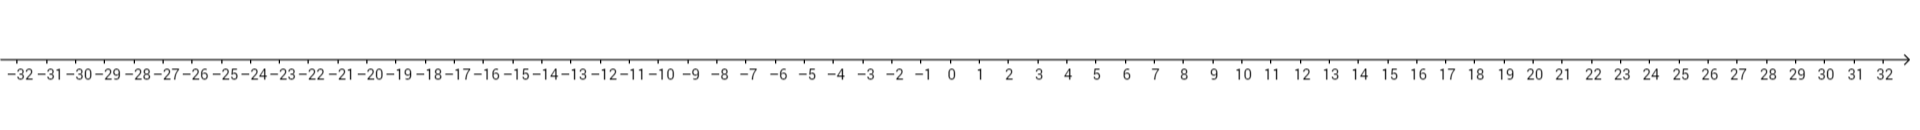
\includegraphics[width=1.3\textwidth]{line2}
\item
\(t=0\), \(t=1\), \(t=2\), \(t=5\), \(t=9\)일 때의 \(P\)의 좌표인 \(x(0)\), \(x(1)\), \(x(2)\), \(x(5)\), \(x(9)\)를 구하여라.\\
\(x(0)=\pb{1},\quad x(1)=\pb{1},\quad x(2)=\pb{1},\quad x(5)=\pb{1},\quad x(9)=\pb{1}\)
\item
\(0\)초부터 \(10\)초까지 \(P\)의 평균 속도를 구하여라.\\
\(v_{0\sim10}=\pb{1}\)
\item
\(t=1\), \(t=2\), \(t=5\), \(t=9\)일 때의 \(P\)의 순간속도인 \(v(1)\), \(v(2)\), \(v(5)\), \(v(9)\)를 구하여라.\\
\(v(0)=\pb{1},\quad v(1)=\pb{1},\quad v(2)=\pb{1},\quad v(5)=\pb{1},\quad v(9)=\pb{1}\)
\item
시간에 따른 위치의 그래프(\(x-t\)그래프)와 \\시간에 따른 속도의 그래프(\(v-t\)그래프)를 나타내어라.\\\\
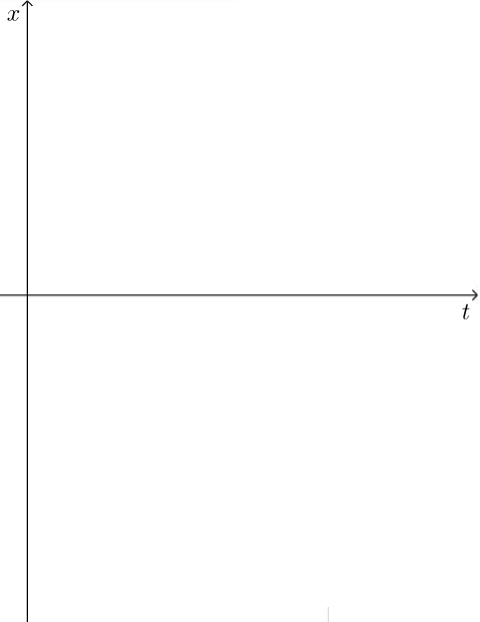
\includegraphics[width=0.37\textwidth]{xt}\qquad\qquad
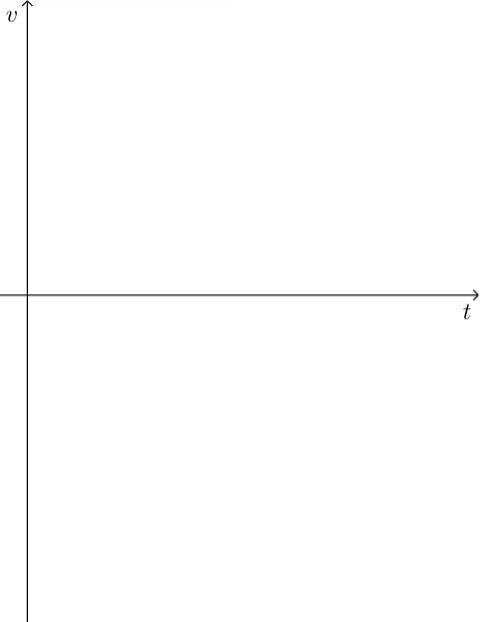
\includegraphics[width=0.37\textwidth]{vt}
\item
시각 \(t\)에서의 \(P\)의 위치 \(x(t)\)와 \(P\)의 속도 \(v(t)\)를 \(t\)에 대한 식으로 나타내어라.\\
\(x(t)=\pb{111},\qquad v(t)=\pb{1}\)
\end{enumerate}


%
\exam{}
\(x=10\)을 출발하여 수직선 위를 움직이는 점 \(P\)가 \(0\le t\le 10\)의 시간동안 \(4\)의 속력으로 왼쪽으로 운동한다.
\begin{enumerate}[label=(\(\arabic*\))]
\item
아래 수직선 상에 \(t=0\), \(t=1\), \(t=2\), \(t=5\), \(t=9\)일 때의 \(P\)의 위치를 \(P_0\), \(P_1\), \(P_2\), \(P_5\), \(P_9\) 등으로 표시하여라.\\
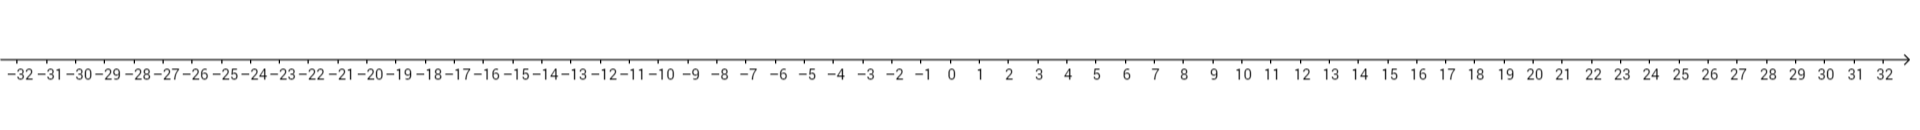
\includegraphics[width=1.3\textwidth]{line2}
\item
\(t=0\), \(t=1\), \(t=2\), \(t=5\), \(t=9\)일 때의 \(P\)의 좌표인 \(x(0)\), \(x(1)\), \(x(2)\), \(x(5)\), \(x(9)\)를 구하여라.\\
\(x(0)=\pb{1},\quad x(1)=\pb{1},\quad x(2)=\pb{1},\quad x(5)=\pb{1},\quad x(9)=\pb{1}\)
\item
\(0\)초부터 \(10\)초까지 \(P\)의 평균속도를 구하여라.\\
\(v_{0\sim10}=\pb{1}\)
\item
\(t=1\), \(t=2\), \(t=5\), \(t=9\)일 때의 \(P\)의 순간속도인 \(v(1)\), \(v(2)\), \(v(5)\), \(v(9)\)를 구하여라.\\
\(v(0)=\pb{1},\quad v(1)=\pb{1},\quad v(2)=\pb{1},\quad v(5)=\pb{1},\quad v(9)=\pb{1}\)
\item
\(x-t\)그래프와 \(v-t\)그래프를 각각 나타내어라.\\\\
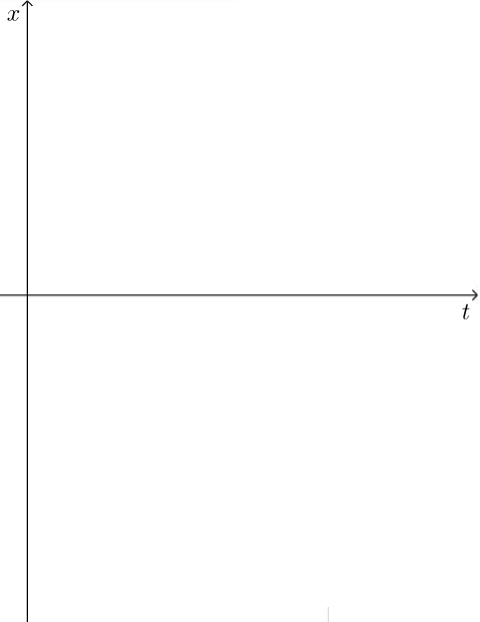
\includegraphics[width=0.4\textwidth]{xt}\qquad\qquad
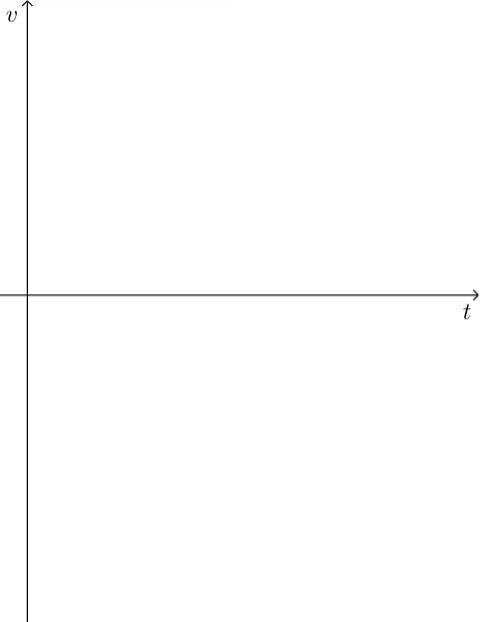
\includegraphics[width=0.4\textwidth]{vt}
\item
시각 \(t\)에서의 \(P\)의 위치 \(x(t)\)와 \(P\)의 속도 \(v(t)\)를 \(t\)에 대한 식으로 나타내어라.\\
\(x(t)=\pb{111},\qquad v(t)=\pb{1}\)
\end{enumerate}

\clearpage
%
\exam{}
원점을 출발하여 수직선 위를 움직이는 점 \(P\)가 \(0\le t\le 5\)의 시간 동안에는 \(4\)의 속력으로 왼쪽으로 움직이다가, \(5\le t\le 10\)의 시간 동안에는 \(3\)의 속력으로 오른쪽으로 운동한다.
\begin{enumerate}[label=(\(\arabic*\))]
\item
아래 수직선 상에 \(t=0\), \(t=1\), \(t=2\), \(t=5\), \(t=9\)일 때의 \(P\)의 위치를 \(P_0\), \(P_1\), \(P_2\), \(P_5\), \(P_9\) 등으로 표시하여라.\\
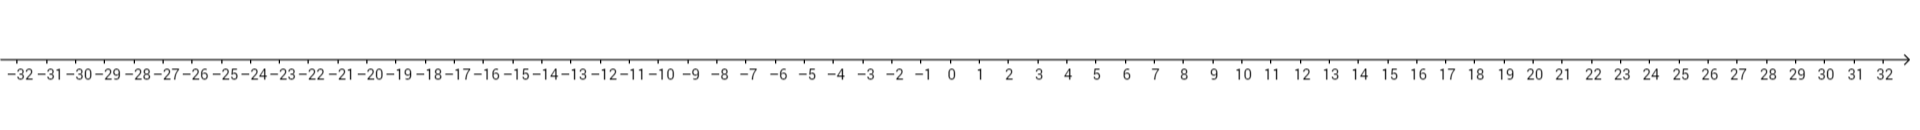
\includegraphics[width=1.3\textwidth]{line2}
\item
\(t=0\), \(t=1\), \(t=2\), \(t=5\), \(t=9\)일 때의 \(P\)의 좌표인 \(x(0)\), \(x(1)\), \(x(2)\), \(x(5)\), \(x(9)\)를 구하여라.\\
\(x(0)=\pb{1},\quad x(1)=\pb{1},\quad x(2)=\pb{1},\quad x(5)=\pb{1},\quad x(9)=\pb{1}\)
\item
\(0\)초부터 \(10\)초까지 \(P\)의 평균속도를 구하여라.\\
\(v_{0\sim10}=\pb{1}\)
\item
\(t=1\), \(t=2\), \(t=5\), \(t=9\)일 때의 \(P\)의 순간속도인 \(v(1)\), \(v(2)\), \(v(5)\), \(v(9)\)를 구하여라.\\
\(v(0)=\pb{1},\quad v(1)=\pb{1},\quad v(2)=\pb{1},\quad v(5)=\pb{1},\quad v(9)=\pb{1}\)
\item
\(x-t\)그래프와 \(v-t\)그래프를 각각 나타내어라.\\\\
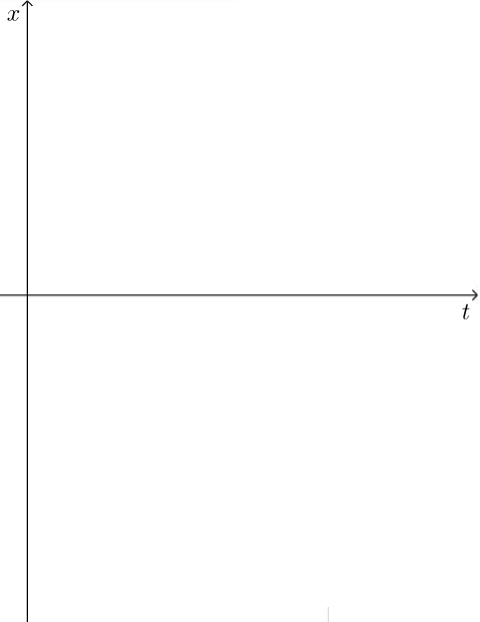
\includegraphics[width=0.4\textwidth]{xt}\qquad\qquad
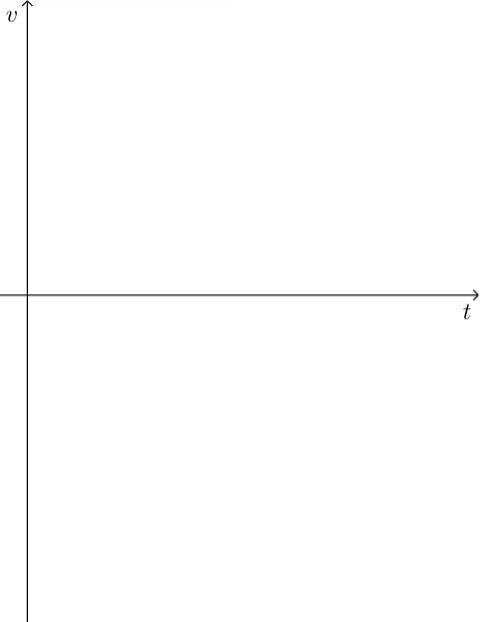
\includegraphics[width=0.4\textwidth]{vt}
\item
시각 \(t\)에서의 \(P\)의 위치 \(x(t)\)와 \(P\)의 속도 \(v(t)\)를 \(t\)에 대한 식으로 나타내어라.\\
\(x(t)=\begin{cases}\pb{111}&(0<t<5)\\\pb{111}&(5<t<10)\end{cases},\qquad
v(t)=\begin{cases}\pb{111}&(0<t<5)\\\pb{111}&(5<t<10)\end{cases}\)
\end{enumerate}

\clearpage
%
\exam{}
원점을 출발하여 수직선 위를 움직이는 점 \(P\)가 \(0\le t\le 3\)의 시간 동안에는 \(10\)의 속력으로 오른쪽으로 움직이다가, \(3\le t\le 6\)의 시간 동안에는 정지해있고, 다시 \(6\le t\le 10\)의 시간 동안에는 \(10\)의 속력으로 왼쪽으로 운동한다.
\begin{enumerate}[label=(\(\arabic*\))]
\item
아래 수직선 상에 \(t=0\), \(t=1\), \(t=2\), \(t=5\), \(t=9\)일 때의 \(P\)의 위치를 \(P_0\), \(P_1\), \(P_2\), \(P_5\), \(P_9\) 등으로 표시하여라.\\
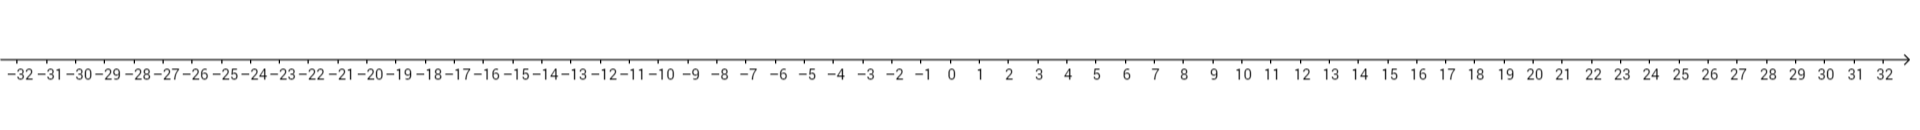
\includegraphics[width=1.3\textwidth]{line2}
\item
\(t=0\), \(t=1\), \(t=2\), \(t=5\), \(t=9\)일 때의 \(P\)의 좌표인 \(x(0)\), \(x(1)\), \(x(2)\), \(x(5)\), \(x(9)\)를 구하여라.\\
\(x(0)=\pb{1},\quad x(1)=\pb{1},\quad x(2)=\pb{1},\quad x(5)=\pb{1},\quad x(9)=\pb{1}\)
\item
\(0\)초부터 \(10\)초까지 \(P\)의 평균속도를 구하여라.\\
\(v_{0\sim10}=\pb{1}\)
\item
\(t=1\), \(t=2\), \(t=5\), \(t=9\)일 때의 \(P\)의 순간속도인 \(v(1)\), \(v(2)\), \(v(5)\), \(v(9)\)를 구하여라.\\
\(v(1)=\pb{1},\quad v(2)=\pb{1},\quad v(5)=\pb{1},\quad v(9)=\pb{1}\)
\item
\(x-t\)그래프와 \(v-t\)그래프를 각각 나타내어라.\\\\
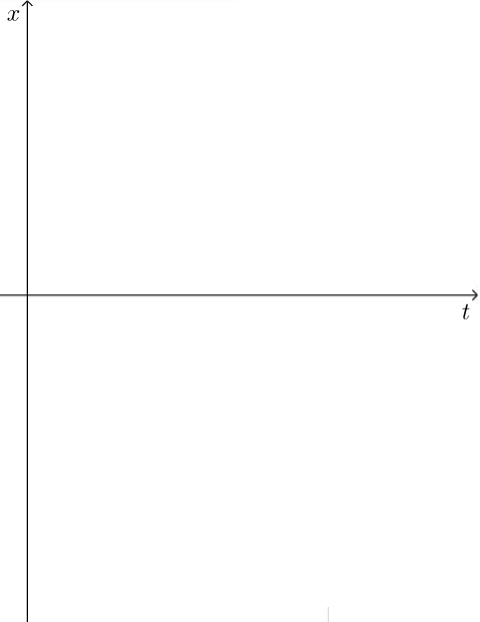
\includegraphics[width=0.4\textwidth]{xt}\qquad\qquad
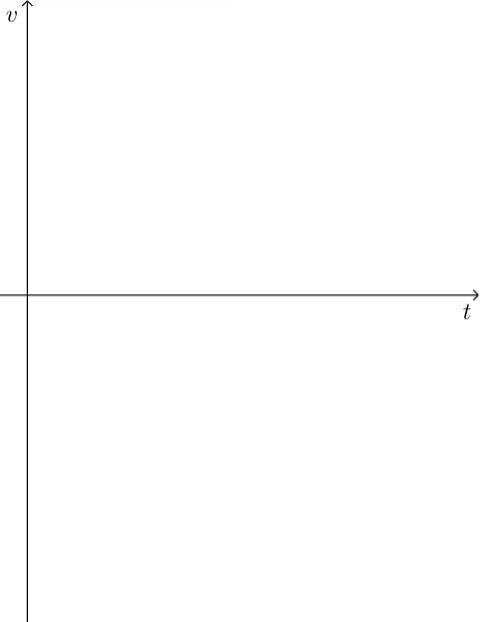
\includegraphics[width=0.4\textwidth]{vt}
\item
시각 \(t\)에서의 \(P\)의 위치 \(x(t)\)와 \(P\)의 속도 \(v(t)\)를 \(t\)에 대한 식으로 나타내어라.\\
\(x(t)=\qquad\qquad\qquad\qquad\qquad\qquad
v(t)=\)
\end{enumerate}

\clearpage
%
\exam{}
원점을 출발하여 수직선 위를 움직이는 점 \(P\)의 시간 \(t\)에서의 좌표가
\[x(t)=20t-5t^2\]
로 주어진다.
\begin{enumerate}[label=(\(\arabic*\))]
\item
아래 수직선 상에 \(t=0\), \(t=1\), \(t=2\), \(t=3\), \(t=4\)일 때의 \(P\)의 위치를 \(P_0\), \(P_1\), \(P_2\), \(P_3\), \(P_4\) 등으로 표시하여라.\\
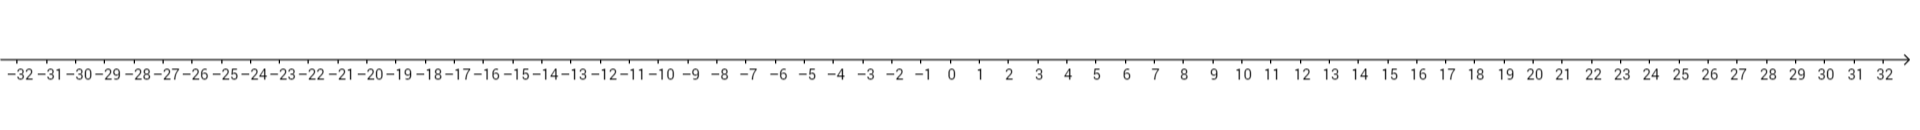
\includegraphics[width=1.3\textwidth]{line2}
\item
\(t=0\), \(t=1\), \(t=2\), \(t=3\), \(t=4\)일 때의 \(P\)의 좌표인 \(x(0)\), \(x(1)\), \(x(2)\), \(x(3)\), \(x(4)\)를 구하여라.\\
\(x(0)=\pb{1},\quad x(1)=\pb{1},\quad x(2)=\pb{1},\quad x(5)=\pb{1},\quad x(9)=\pb{1}\)
\item
\(x-t\)그래프를 나타내어라.\\\\
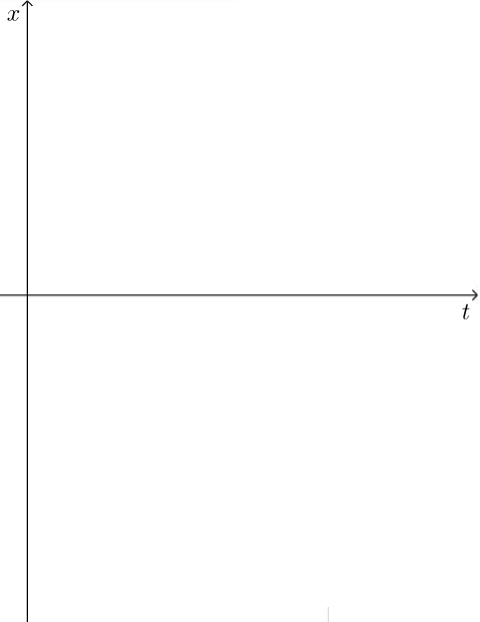
\includegraphics[width=0.4\textwidth]{xt}
\item
\(0\)초부터 \(3\)초까지 \(P\)의 평균속도를 구하여라.\\
\(v_{0\sim3}=\pb{1}\)
\item
\(t=1\), \(t=2\) 순간속도인 \(v(1)\), \(v(2)\)을 유추하여라.\\
\(v(1)=\pb{1},\quad v(2)=\pb{1}\)
\end{enumerate}

\clearpage
%
\exam{}
수직선 위를 움직이는 점 \(P\)의 시간 \(t\)에서의 좌표가
\[x(t)=-5t^2+10t+15\]
로 주어진다.
\begin{enumerate}[label=(\(\arabic*\))]
\item
아래 수직선 상에 \(t=0\), \(t=1\), \(t=2\), \(t=3\), \(t=4\)일 때의 \(P\)의 위치를 \(P_0\), \(P_1\), \(P_2\), \(P_3\), \(P_4\) 등으로 표시하여라.\\
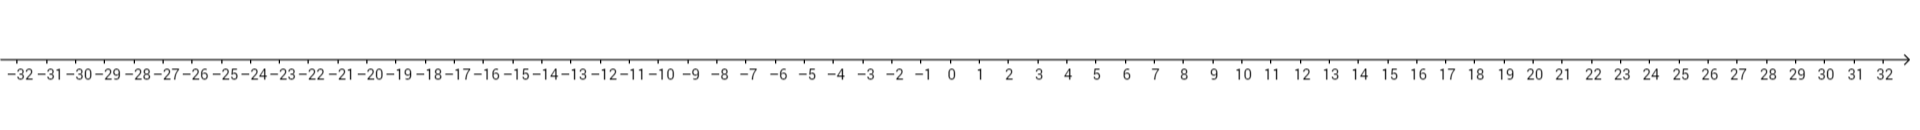
\includegraphics[width=1.3\textwidth]{line2}
\item
\(t=0\), \(t=1\), \(t=2\), \(t=3\), \(t=4\)일 때의 \(P\)의 좌표인 \(x(0)\), \(x(1)\), \(x(2)\), \(x(3)\), \(x(4)\)를 구하여라.\\
\(x(0)=\pb{1},\quad x(1)=\pb{1},\quad x(2)=\pb{1},\quad x(5)=\pb{1},\quad x(9)=\pb{1}\)
\item
\(x-t\)그래프를 나타내어라.\\\\
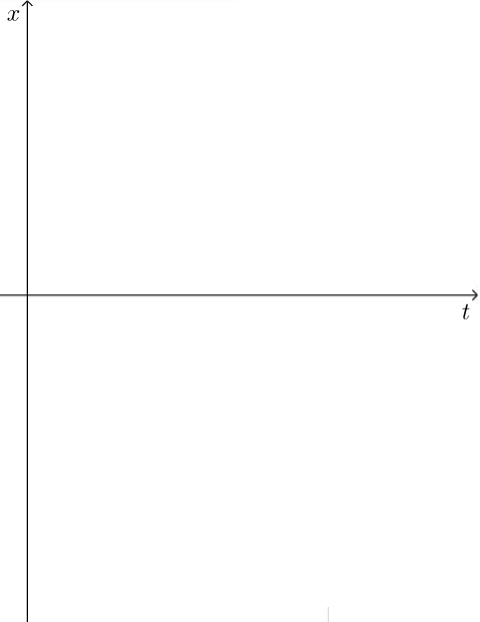
\includegraphics[width=0.4\textwidth]{xt}
\item
\(0\)초부터 \(3\)초까지 \(P\)의 평균속도를 구하여라.\\
\(v_{0\sim3}=\pb{1}\)
\item
\(t=1\), \(t=2\) 순간속도인 \(v(1)\), \(v(2)\)을 유추하여라.\\
\(v(1)=\pb{1},\quad v(2)=\pb{1}\)
\end{enumerate}

%%
\section{미분계수}
\begin{mdframed}
%
\defi{평균변화율}
함수 \(y=f(x)\)에서 \(x\)의 값이 \(a\)에서 \(b\)까지 변할 때의 \emph{평균변화율}은
\[\frac{\Delta y}{\Delta x}=\frac{f(b)-f(a)}{b-a}=\frac{f(a+\Delta x)-f(a)}{\Delta x}\]
이다.
\begin{center}
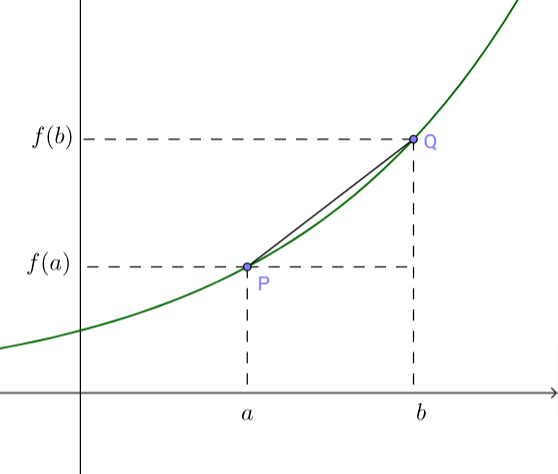
\includegraphics[width=0.5\textwidth]{average_rate_of_change}
\end{center}
\end{mdframed}
\(*\) 위의 그림 상에 \(\Delta x\)와 \(\Delta y\)를 각각 표시하시오.\\
\(**\) 이때 \(\Delta x\) 대신 \(h\)를 쓰기도 한다.
\bigskip

%
\exam{}
함수 \(f(x)=x^2\)가 \(0\)에서 \(3\)까지 변할 때의 평균변화율은
\[
\frac{\Delta y}{\Delta x}=\frac{f(3)-f(0)}{3-0}=\frac{9-0}{3}=3
\]
이다.

\bigskip
`평균변화율'은 위치와 속도에서 나왔던 `평균속도'의 의미와 비슷하다.
위치와 속도에서 나왔던 `순간속도'의 의미와 비슷한 것은 다음의 `순간변화율'이다.

\begin{center}
\begin{tabu}spread 0pt {|X[c]|X[c]|}\hline
평균속도	&순간속도\\\hline
평균변화율	&순간변화율(=미분계수)\\\hline
\end{tabu}
\end{center}

\begin{mdframed}
%
\defi{순간변화율(미분계수)}
함수 \(y=f(x)\)의 \(x=a\)에서의 \emph{순간변화율(미분계수)} \(f'(a)\)는
\[f'(a)=\lim_{\Delta x\to0}\frac{\Delta y}{\Delta x}=\lim_{\Delta x\to0}\frac{f(a+\Delta x)-f(a)}{\Delta x}=\lim_{\pb{aaa}}\frac{f(x)-f(a)}{x-a}\]
이다.
\begin{center}
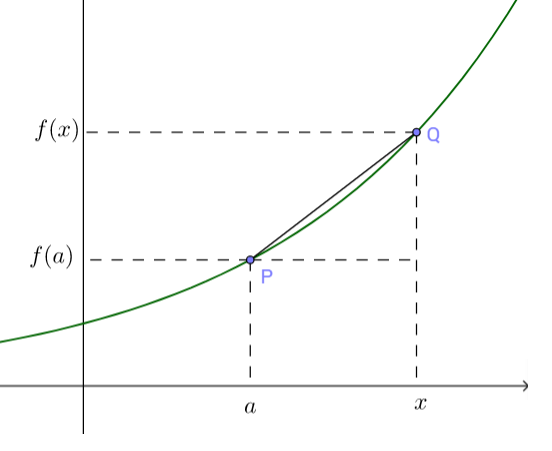
\includegraphics[width=0.5\textwidth]{differential_coefficient}
\end{center}
\end{mdframed}
\(*\) 위의 그림 상에 \(\Delta x\)와 \(\Delta y\)를 각각 표시하시오.\\
\(**\) 이때 \(\Delta x\) 대신 \(h\)를 쓰기도 한다.\\
\(***\) 위의 극한식의 빈칸에 알맞은 것을 넣으시오.
\bigskip

%
\exam{}
함수 \(f(x)=x^2\)의 \(x=1\)에서의 순간변화율(미분계수) \(f'(1)\)은
\begin{align*}
f'(1)
&=\lim_{\Delta x\to0}\frac{f(1+\Delta x)-f(1)}{\Delta x}\\
&=\lim_{\Delta x\to0}\frac{(1+\Delta x)^2-1^2}{\Delta x}\\
&=\lim_{\Delta x\to0}\frac{\{1+2\Delta x+(\Delta x)^2\}-1^2}{\Delta x}\\
&=\lim_{\Delta x\to0}\frac{(\Delta x)^2+2\Delta x}{\Delta x}\\
&=\lim_{\Delta x\to0}\left(\Delta x+2\right)\\
&=2
\end{align*}
와 같이 계산할 수 있다.
이때 \(\Delta x\)와 같은 기호는 조금 쓰기가 번거로울 수 있으므로 \(h\)로 바꿔서 쓰면 훨씬 편하다.
또한 다음과 같이 계산할 수도 있다.
\begin{align*}
f'(1)
&=\lim_{x\to1}\frac{f(x)-f(1)}{x-1}\\
&=\lim_{x\to1}\frac{x^2-1^2}{x-1}\\
&=\lim_{x\to1}\frac{(x+1)(x-1)}{x-1}\\
&=\lim_{x\to1}(x+1)\\
&=2
\end{align*}
따라서, 두 계산값이 똑같다는 것을 확인할 수 있다.

\bigskip
순간변화율(미분계수)는 평균변화율의 극한이다.
평균변화율은 두 점 사이의 기울기이므로, 순가변화율(미분계수)는 기울기의 극한값이라고 생각할 수 있다.
따라서 이 예시에서 \(f'(1)\)의 의미는 `\(y=x^2\)의 \(P(1,1)\)에서의 접선의 기울기'이다.
\begin{mdframed}[leftmargin=60pt,rightmargin=60pt,innertopmargin=10pt,innerbottommargin=10pt]
\begin{center}
순간변화율(미분계수)=접선의 기울기
\end{center}
\end{mdframed}

\begin{figure*}[h!]
\centering
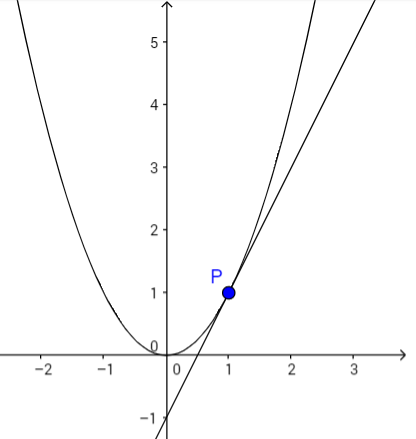
\includegraphics[width=0.5\textwidth]{differential_coefficient_example}
\end{figure*}


%%\section{미분가능성}
%%\section{도함수}

\end{document}